\documentclass[12pt, letterpaper]{article}
\usepackage{graphicx} % Required for inserting images
\usepackage{hyperref}
\usepackage{listings}
\usepackage{amssymb}
\usepackage{amsmath}
\usepackage[english]{babel}
\usepackage{nicefrac, xfrac}
\usepackage{mathtools}
\newcommand{\acc}{\\\hphantom{}\\}
\usepackage[dvipsnames]{xcolor}
\usepackage[table,xcdraw]{xcolor}
\definecolor{light-gray}{gray}{0.95}
\newcommand{\code}[1]{\colorbox{light-gray}{\texttt{#1}}}
\newcommand{\codee}[1]{\colorbox{white}{\texttt{#1}}}
\usepackage[paper=a4paper,left=20mm,right=20mm,bottom=25mm,top=25mm]{geometry}
\renewcommand{\labelenumii}{\arabic{enumi}.\arabic{enumii}}
\renewcommand{\labelenumiii}{\arabic{enumi}.\arabic{enumii}.\arabic{enumiii}}
\renewcommand{\labelenumiv}{\arabic{enumi}.\arabic{enumii}.\arabic{enumiii}.\arabic{enumiv}}
\newcommand{\id}{{\hphantom{ident}}}
\newcommand{\vincolo}[1]{\colorbox{Orange}{$[$\text{#1}$]$}}
\title{\textbf{eBuy}}

\date{}


\begin{document}

\maketitle\section{Requisiti}
\hphantom{a}\\
1.  \textbf{Utente}\\
\id	1.1 nome\\
\id	1.2 data registrazione\\
\id	1.3 id\\
\id 1.4 affidabilità\\
\acc
2.  \textbf{Post} (annuncio)\\
\id2.1 descrizione oggetto\\
\id2.2 categoria (fai classe categoria)\\
\id	2.3 garanziaInAnni int$\ge$0\\
\id	2.4 pagabile in (implementato con enum)\\
\id\id		2.4.1 bonifico\\
\id\id		2.4.2 carta di credito\\
\id	2.5 usato? (implementato con enum)\\
\id\id		2.5.1 nuovo\\
\id\id\id			2.5.1.1 garanziaInAnni int$>$1 (attributo specializzato)\\
\id\id	2.5.2 usato\\
\id\id\id		2.5.2.1 condizioni {ottimo,buono,discreto, da sistemare}\\
\id2.6 asta o no? (disjoint.complete)\\
\id\id		2.6.1 post con asta\\
\id\id\id		2.6.1.1 prezzo iniziale in (euro,centesimi)\\
\id\id\id		2.6.1.2 prezzo rialzi in (euro,centesimi)\\
\id\id\id		2.6.1.3 istante scadenza asta (date time)\\
\id\id\id		2.6.1.4 insieme di Bid (offerte)\\
\id\id	2.6.2 post senza asta\\
        \id\id\id		2.6.2.1 prezzo in (euro,centesimi)\\
        \id\id\id		2.6.2.1 utente che ha effettuato l'acquisto\\
\acc
3. \textbf{Bid} (offerta)\\
\id	3.1 Utente che ha fatto l'offerta\\
\id	3.2 Post in questione\\
    \id	3.3 Istante offerta \\
    \id	3.4 ordine nell'offerta, n se è l'n-esimo utente che fa l'offerta\\
    \id	3.5 prezzo offerta = n$\cdot$Post.rialzo+prezzo iniziale\\
4. \textbf{Venditore Professionale} - sottoclasse di \textit{Utente}\\
\id 4.4 urlVetrina\\
\id 4.5 popolarità\\
\acc
\section{Diagramma UML}\begin{center}
    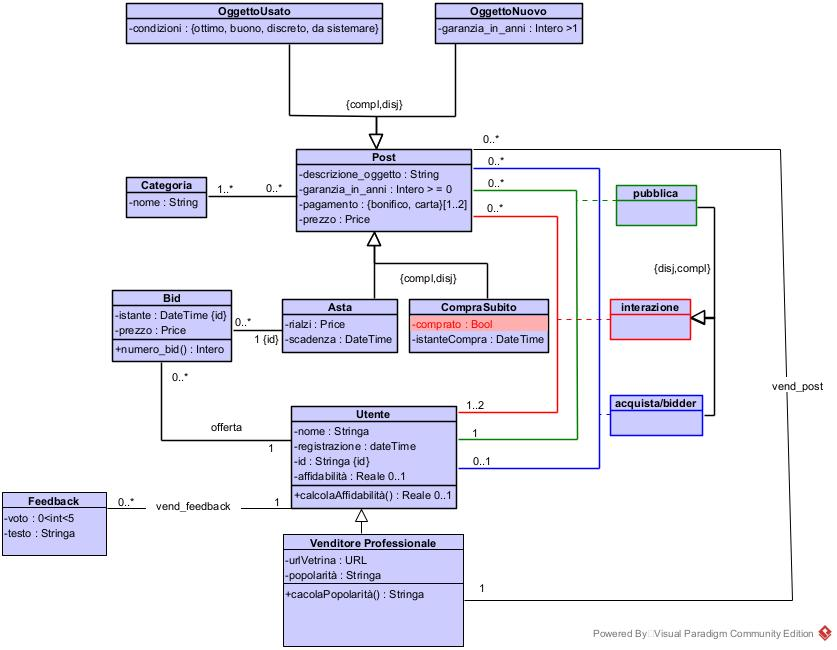
\includegraphics[width=\textwidth ]{UML.jpg}
\end{center}
\newpage
\section{Diagramma Use-Case}\begin{center}
    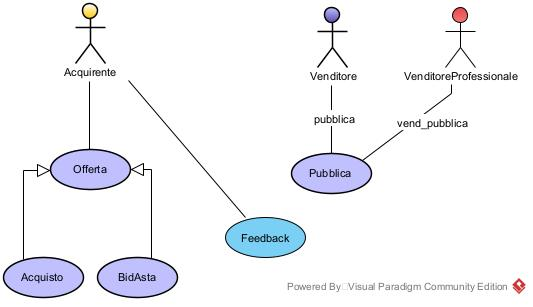
\includegraphics[width=\textwidth ]{useCase.jpg}\acc
\end{center}

\section{Specifiche}
\subsection{Specifica dei tipi di dato}
Price = (euro : Int$>$0, cent : $[$0..99$]$ ) \\
URL = \{'https://',Stringa,'$.$',Stringa[2]\}\newpage
\subsection{Specifica delle classi}
\subsubsection{Bid}
\code{numero\_bid () : Intero}\begin{itemize}
    \item \textit{pre-condizioni} : Nessuna
    \item \textit{post-condizioni} : Non modifica il livello degli oggetti.\\ 
    Sia $a:Asta$ l'oggetto per cui esiste il link ($this,a$)\\ 
    Sia $B$ l'insieme di tutti gli oggetti $x:Bid$ per cui $\exists (x,a) \land x.istante<this.istante$\\ 
    $result = |B|+1$ 
\end{itemize}
\subsubsection{Venditore Professionale}
\code{cacolaPopolarità () : Stringa}\begin{itemize}
    \item \textit{pre-condizioni} : Nessuna
    \item \textit{post-condizioni} : \\Sia insPostAsta l'insieme degli oggetti $p:Post$ per cui $\exists (this,p):vend\_post$ e Post è di tipo Asta con scadenza $<$ now per cui $\exists$ almeno un Bid con Bid.instante $<=$ now- 12mesi.\acc
                                    Sia insPostComprSub l'insieme degli oggetti $p:Post$ per cui $\exists (this,p):vend\_post$ e Post è di tipo CompraSubito con CompraSubito.comprato = True e CompraSubito.istanteCompra è $<=$ now- 12mesi.\acc
                                    Inserisco negli insiemi solo Bid o Acquisti di \textbf{utenti diversi}\\ $\rightarrow \not \exists$ u1: Utente = u2:Utente in InsPostAsta o in insPosComprSub. \\
                                    Sia Tot= $|$insPostAsta$|+|$insPostComprSub$|$\\
                                    Imposta VenditoreProfessinale.popolarità=\\ "Bassa" se Tot$<$50, "Media" se 50$\le$Tot$<$300, "Alta" se Tot$\ge$300

\end{itemize}
\subsubsection{Utente}
\code{calcolaAffidabilità(): Reale 0..1} \begin{itemize}
    \item \textit{pre-condizioni} : $\exists p:Post$ per cui $\exists (this,p):pubblica$ e $p$ è di tipo CompraSubito e $p.comprato=True$ $\lor$ $\exists p:Post$ per cui $\exists (this,p):pubblica$ e $p$ è di tipo Asta e $p.scadenza>now$ $\land$ $\exists$ almeno un bid.
    \item \textit{post-condizioni} : Sia insFeed l'insieme degli oggetti Feedback legati a this con un link $(this,Feedback): vend\_feedback$, lasciati all'utente.\\
    Sia $m$ la media aritmetica di tutti i Feedback.voto che ha ricevuto, sia $z$ la frazione dei Feedback.voto negativi rispetto ai feedback totali.\\
    Ritorna $m(1-z)/5$.\\
\end{itemize}
Questa operazione è ereditata dalla sottoclasse VenditoreProfessinale.\\
\textbf{Attenzione}\\
L'operazione feedback è specificata nella specifica degli use-case.
\subsection{Specifica dei vincoli esterni}
\vincolo{V.Bid.istante\_offerta} : $\forall b:Bid$  e $\forall a:Asta$ per cui $\exists (a,b)$, deve 
essere vero che $b.istante\le a.scadenza$.\acc
\vincolo{V.Bid.istante\_reg\_utente} :  $\forall b:Bid$  e $\forall u:Utente$ per cui $\exists (u,b)$, deve 
essere vero che $b.istante\ge u.registrazione$.\acc
\vincolo{V.Utente.scadenza\_aste} : $\forall u:Utente$, sia $P$ l'insieme degli oggetti $p:Asta$ tale che 
$\exists (p,u):vende$. $\forall p\in P$ deve essere vero che $p.scadenza\ge u.registrazione$.\acc 
\vincolo{V.VenditoreProfessinale.scadenza\_aste} : $\forall u:Utente$, sia $P$ l'insieme degli oggetti $p:Asta$ tale che 
$\exists (p,u):vende$. $\forall p\in P$ deve essere vero che $p.scadenza\ge u.registrazione$.\acc 

\subsection{Specifica degli use-case}
\subsubsection{Acquirente}
\textbf{Offerta}\\
\code{BidAsta (a:Asta, u:Utente) :  Bid }\begin{itemize}
    \item \textit{pre-condizioni} : Non deve esistere $(u,a):pubblica$. 
    \item \textit{post-condizioni} : Viene creato un oggetto $b:Bid$ tale che:\\ 
     $b.istante=now$ \\
     $\exists (u,b) : offerta$ \\
     $\exists (a,b) $ \\ 
     Sia $r=a.rialzi$\\ 
     Sia $price=a.prezzo$\\
     $b.prezzo = price + r\cdot ($\codee{this.numero\_bid()} $-1 )$\\
     Viene creato $(u,a):acquista/bidder$ 
\end{itemize}
\code{Acquisto (c:CompraSubito, u:Utente) }\begin{itemize}
    \item \textit{pre-condizioni} : Non deve esistere $(u,c):pubblica$, non deve 
    esistere un link di tipo $acquista$ in cui è coinvolto $c$. 
    \item \textit{post-condizioni} : Viene creato un link di tipo $(u,c):scquista/bidder$, viene inoltre settato CompraSubito.comprato=True e istanteCompra=now.\\
\end{itemize}

\textbf{Feedback}\\
\code{Feedback}\begin{itemize}
    \item \textit{pre-condizioni} : L'utente ha effettuato un use-case tra Acquisto o  BidAsta il cui instante è l'ultimo prima di Asta.scadenza, ovvero ha acquistato l'oggetto.
    \item \textit{post-condizioni}: L'utente può lasciare un voto da 0 a 5 (intero) e un feedback testuale, viene creato un nuovo link (venditore,feedback): vend\_feedback \textit{(per venditore si intende l'utente/ venditoreProfessinale che ha inserito il post acquistato dall'utente)}.\\
    L'oggetto di tipo feedback avrà come Feedback.voto il valore scelto dall'utente e Feedback.testo il testo scritto dall'utente.
\end{itemize}
\subsubsection{Venditore}
\textbf{Pubblica}\\
\code{ pubblica ( u : Utente, prezzoIniziale : Price, desc :Stringa, gar : Intero$>$1,
}\\\code{ pag : \{Bonifico,Carta\}[1..2],
rialzi : Price, scad : DateTime$> now$,}\\\code{ cat : Categoria[1..*])}\begin{itemize}
    \item \textit{pre-condizioni} : Deve esistere almeno un oggetto di tipo Categoria.
    \item \textit{post-condizioni} : Viene creato un oggetto $a:Asta$ tale che\\ 
    $a.Price = prezzoIniziale$\\ 
    $a.descrizione\_oggetto = desc$\\ 
    $a.garanzia\_in\_anni = gar$\\ 
    $a.pagamento = pag$\\
    $\forall c \in cat$, crea un link $(a,c)$\\
    $a.scadenza=sca$ \\
    $a.rialzi=rialzi$\\
    Viene creato un link $(u,a):pubblica$.
\end{itemize}
Simile ed analogo per i metodi realativi al:\begin{itemize}
    \item Creare un post (compra subito) per un oggetto usato 
    \item Creare un post (compra subito) per un oggetto nuovo 
    \item Creare un asta per un oggetto usato
\end{itemize}


\subsubsection{Venditore Professionale}
\textbf{Pubblica}\\
\code{ creaAstaNuovo ( u : Utente, prezzoIniziale : Price, desc :Stringa, gar : Intero$>$1,
}\\\code{ pag : \{Bonifico,Carta\}[1..2],
rialzi : Price, scad : DateTime$> now$,}\\\code{ cat : Categoria[1..*])}\begin{itemize}
    \item \textit{pre-condizioni} : Deve esistere almeno un oggetto di tipo Categoria.
    \item \textit{post-condizioni} : Viene creato un oggetto $a:Asta$ tale che\\ 
    $a.Price = prezzoIniziale$\\ 
    $a.descrizione\_oggetto = desc$\\ 
    $a.garanzia\_in\_anni = gar$\\ 
    $a.pagamento = pag$\\
    $\forall c \in cat$, crea un link $(a,c)$\\
    $a.scadenza=sca$ \\
    $a.rialzi=rialzi$\\
    Viene creato un link $(u,a):pubblica$.
\end{itemize}
Simile ed analogo per i metodi realativi al:\begin{itemize}
    \item Creare un post (compra subito) per un oggetto usato 
    \item Creare un post (compra subito) per un oggetto nuovo 
    \item Creare un asta per un oggetto usato
\end{itemize}


\end{document}